The Iterative Model Solution (IMS) solves the nonlinear groundwater flow equations of a Newton--Raphson formulation with nested iterations: each outer iteration forms a linear system for the head change, and inner iterations of a preconditioned Krylov method (conjugate gradient or BiCGSTAB) solve that system approximately \citep{modflow6framework}. The inner iterations stop when the change in head and the residual fall below \texttt{INNER\_DVCLOSE} and \texttt{INNER\_RCLOSE}, or when \texttt{INNER\_MAXIMUM} iterations have been taken. In large Newton--Raphson models the second condition is reached in most outer iterations, so the accuracy of each linear solve, and with it the head change applied to the model, is set by the iteration limit rather than by a tolerance. When a model is solved in parallel, the preconditioner depends on how the model is divided among processors, so a fixed number of inner iterations gives a different head change for each division, and simulations that differ only in the number of processors follow different sequences of outer iterations to the same solution.

This chapter summarizes the inexact Newton literature that applies to this behavior and describes the Eisenstat--Walker forcing terms and backtracking test added to IMS as options. With the \texttt{FORCING\_TERMS} option the accuracy of each linear solve is tied to the progress of the outer iterations, and with the \texttt{BACKTRACKING\_SUFFICIENT\_DECREASE} option the backtracking acceptance test is also tied to that accuracy. Both options apply only to solutions that contain a model using the Newton--Raphson formulation, and neither is used by default, because on a small problem with drying and rewetting cells they conflict with delta-bar-delta under-relaxation, the under-relaxation used by \texttt{COMPLEXITY COMPLEX}.

\subsection{Partition-Dependent Convergence}

The behavior was examined with a large regional steady-state model using the Newton--Raphson formulation, with about 125 million cells divided among 256 models and solved in parallel with BiCGSTAB, block Jacobi preconditioning, and an incomplete LU factorization with threshold (ILUT) on each processor's block. Pseudo-transient continuation, delta-bar-delta under-relaxation, backtracking, and Newton under-relaxation were active, and \texttt{INNER\_MAXIMUM} was 50. Run with 32, 64, 128, and 256 processors, the model required 484, 372, 402, and 437 outer iterations and 12,820, 9,715, 10,631, and 12,510 inner iterations, although every run solved the same equations from the same starting heads.

The divergence of the four runs starts with round-off. The residual entering the second outer iteration differed between processor counts by a relative amount of about $10^{-6}$; by outer iterations 22 to 27 the difference was about $10^{-2}$. The backtracking decisions were the same for every processor count until outer iteration 56, so backtracking amplified a divergence that had already begun rather than causing it.

To separate the linear solve from the nonlinear path, the linear system of a single outer iteration was formed once and solved with five divisions of the 256 models among processors: 16, 32, and 64 processors as used in production; 32 processors with four models moved between two processors at a location where the production runs converged slowly (regrouped); and 32 processors with four models moved between two processors elsewhere in the domain (placebo). The system matrix and right-hand side are the same for every division. Systems were formed from the starting heads and from the heads after 100 outer iterations, and each was solved with up to 500 inner iterations (fig.~\ref{fig:imsforcingreplay}). Solved to round-off, the five divisions agree to $1.8 \times 10^{-9}$~m. After 50 inner iterations, the production limit, the heads from the starting-head system differ from the 32-processor heads by up to 0.71~m for 16 processors, 0.088~m for the placebo, 0.010~m for the regrouped division, and 1.23~m for 64 processors; for the system after 100 outer iterations the largest difference is 0.027~m.

\begin{figure}[!ht]
	\centering
	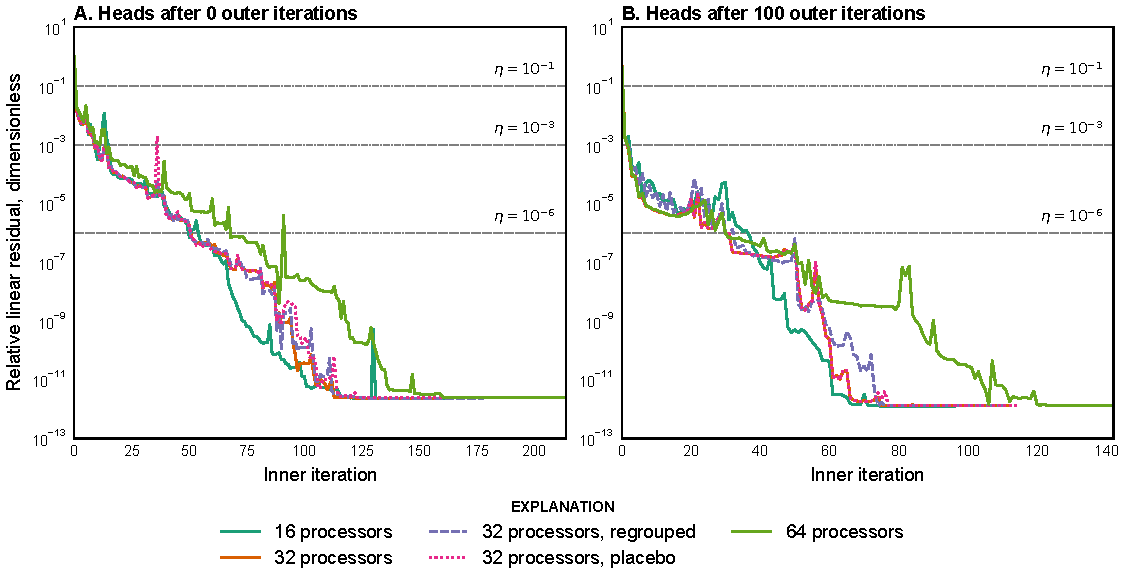
\includegraphics[width=\textwidth]{./Figures/IMSForcingReplay.pdf}
	\caption[Linear residual history of one outer iteration solved with five divisions of a model among processors]{Ratio of the L2 norm of the linear residual to its initial value during the BiCGSTAB solve of one outer iteration of a large regional steady-state model, for five divisions of the model among processors. (\textit{A}) System formed from the starting heads; the L2 norm of the initial residual is $1.098 \times 10^{8}$. (\textit{B}) System formed from the heads after 100 outer iterations; the L2 norm of the initial residual is $8.06 \times 10^{7}$. The matrix and right-hand side are the same for every division within a panel. Horizontal lines mark forcing terms $\eta$ of $10^{-1}$, $10^{-3}$, and $10^{-6}$. The residual is the unpreconditioned residual; each curve levels off near $10^{-12}$, where further reduction is limited by round-off}
	\label{fig:imsforcingreplay}
\end{figure}

Two results follow from figure~\ref{fig:imsforcingreplay}. The 32-processor division is not slower than the others when the nonlinear history is removed, and moving models between processors does not change the inner iterations needed for a given residual reduction (table~\ref{tab:imsforcingits}). The 50-iteration limit, however, reduces the residual of the starting-head system by factors between $7.0 \times 10^{-7}$ and $2.3 \times 10^{-5}$ depending on the division, and of the later system by factors between $5.0 \times 10^{-10}$ and $6.4 \times 10^{-7}$. Each division therefore solves the outer iteration to a different accuracy, and that difference, rather than the linear system, is passed on to the nonlinear path.

\begin{table}[!ht]
	\caption[Inner iterations needed to reduce the linear residual by a forcing term]{Inner iterations needed to reduce the L2 norm of the linear residual of one outer iteration of a large regional steady-state model to the fraction $\eta$ of its initial value, for five divisions of the model among processors}
	\label{tab:imsforcingits}
	\small
	\centering
	\begin{tabular}{l rrrrr rrrrr}
		\hline
		\hline
		& \multicolumn{5}{c}{Starting heads} & \multicolumn{5}{c}{After 100 outer iterations} \\
		\cline{2-6} \cline{7-11}
		Division & $10^{-1}$ & $10^{-2}$ & $10^{-3}$ & $10^{-4}$ & $10^{-6}$ & $10^{-1}$ & $10^{-2}$ & $10^{-3}$ & $10^{-4}$ & $10^{-6}$ \\
		\hline
		16 processors & 1 & 2 & 9 & 17 & 50 & 1 & 1 & 3 & 6 & 37 \\
		32 processors & 1 & 2 & 9 & 19 & 51 & 1 & 1 & 2 & 3 & 30 \\
		32, regrouped & 1 & 2 & 9 & 20 & 51 & 1 & 1 & 3 & 5 & 30 \\
		32, placebo & 1 & 2 & 9 & 19 & 51 & 1 & 1 & 2 & 3 & 30 \\
		64 processors & 1 & 3 & 11 & 26 & 68 & 1 & 1 & 2 & 4 & 30 \\
		\hline
	\end{tabular}
\end{table}

\subsection{Inexact Newton Methods}

For a vector of heads $\mathbf{x}$, the Newton--Raphson formulation solves

\begin{equation}
	\label{eqn:imsf-newton}
	\mathbf{J}(\mathbf{x}_k) \mathbf{s}_k = -\mathbf{F}(\mathbf{x}_k), \qquad \mathbf{x}_{k+1} = \mathbf{x}_k + \mathbf{s}_k ,
\end{equation}

\noindent where $k$ is the outer iteration, $\mathbf{F}$ is the vector of cell flow residuals (L$^3$T$^{-1}$), $\mathbf{J}$ is the Jacobian of $\mathbf{F}$ with respect to head (L$^2$T$^{-1}$), and $\mathbf{s}_k$ is the head change (L). When equation~\ref{eqn:imsf-newton} is solved iteratively, \cite{dembo1982inexact} showed that the outer iterations converge if each linear solve satisfies

\begin{equation}
	\label{eqn:imsf-inexact}
	\| \mathbf{F}(\mathbf{x}_k) + \mathbf{J}(\mathbf{x}_k) \mathbf{s}_k \| \le \eta_k \| \mathbf{F}(\mathbf{x}_k) \| ,
\end{equation}

\noindent where $\eta_k$ is the forcing term (dimensionless) and $\eta_k \le \eta_{\max} < 1$. The convergence of the outer iterations is linear for a fixed forcing term, superlinear if $\eta_k \to 0$, and quadratic if $\eta_k$ decreases in proportion to $\| \mathbf{F}(\mathbf{x}_k) \|$. Equation~\ref{eqn:imsf-inexact} measures the linear solve by the relative reduction of its residual: the left-hand side is the residual remaining after the inner iterations and the right-hand side is a fraction of the residual at the start of the outer iteration. A forcing term that is small far from the solution solves accurately for a head change that is then reduced by under-relaxation or backtracking, which \cite{eisenstat1996forcing} called oversolving. A forcing term that is large near the solution slows the outer iterations.

\cite{eisenstat1996forcing} proposed two forcing terms that follow the progress of the outer iterations. The first compares the residual at the start of the outer iteration with the residual predicted by the previous linear solve,

\begin{equation}
	\label{eqn:imsf-choice1}
	\eta_k = \frac{\left| \| \mathbf{F}(\mathbf{x}_k) \| - \| \mathbf{F}(\mathbf{x}_{k-1}) + \mathbf{J}(\mathbf{x}_{k-1}) \mathbf{s}_{k-1} \| \right|}{\| \mathbf{F}(\mathbf{x}_{k-1}) \|} ,
\end{equation}

\noindent and the second uses only the reduction of the residual between outer iterations,

\begin{equation}
	\label{eqn:imsf-choice2}
	\eta_k = \gamma \left( \frac{\| \mathbf{F}(\mathbf{x}_k) \|}{\| \mathbf{F}(\mathbf{x}_{k-1}) \|} \right)^{\alpha} ,
\end{equation}

\noindent where $\gamma$ is between 0 and 1 and $\alpha$ is between 1 and 2 (dimensionless). Because either choice can become small far from the solution, \cite{eisenstat1996forcing} added safeguards, applied as implemented by \cite{pernice1998nitsol}: for the first choice, $\eta_k$ is replaced by $\max(\eta_k, \eta_{k-1}^{(1+\sqrt{5})/2})$ when $\eta_{k-1}^{(1+\sqrt{5})/2} >$ 0.1, and for the second choice by $\max(\eta_k, \gamma \eta_{k-1}^{\alpha})$ when $\gamma \eta_{k-1}^{\alpha} >$ 0.1; $\eta_k$ is then limited to $\eta_{\max}$. \cite{pernice1998nitsol} start from $\eta_0 =$ 0.5 and use $\eta_{\max} =$ 0.9. \cite{jones2001newton} used the second choice with $\gamma =$ 0.9 and $\alpha =$ 2 for variably saturated flow, and \cite{knoll2004jacobian} review its use with Newton--Krylov methods in other applications.

\cite{eisenstat1994global} made the inexact Newton method converge from starting values far from the solution with a backtracking test that depends on the forcing term. A head change is accepted when

\begin{equation}
	\label{eqn:imsf-sufficient}
	\| \mathbf{F}(\mathbf{x}_k + \mathbf{s}_k) \| \le \left[ 1 - t (1 - \eta_k) \right] \| \mathbf{F}(\mathbf{x}_k) \| ,
\end{equation}

\noindent where $t$ is a small positive number (dimensionless), $10^{-4}$ in \cite{pernice1998nitsol}. Otherwise, the head change and the forcing term are reduced together,

\begin{equation}
	\label{eqn:imsf-reduce}
	\mathbf{s}_k \leftarrow \theta \mathbf{s}_k, \qquad \eta_k \leftarrow 1 - \theta (1 - \eta_k) ,
\end{equation}

\noindent where $\theta$ is a reduction factor between 0 and 1 (dimensionless), and equation~\ref{eqn:imsf-sufficient} is tested again. The reduced head change satisfies equation~\ref{eqn:imsf-inexact} with the reduced forcing term, so the acceptance test always compares the actual residual reduction with the reduction the linear solve was required to deliver. A residual that decreases by less than this, or increases, is not accepted.

Pseudo-transient continuation \citep{kelley1998ptc} adds a storage-like term to the diagonal of $\mathbf{J}$ that is reduced as the residual decreases, using the switched evolution relaxation that IMS also uses. \cite{kelley1998ptc} showed that the method still converges when the linear system is solved inexactly, provided the forcing term is small enough in the intermediate phase between the starting heads and the neighborhood of the solution. Both choices of forcing term are largest in that phase, so the combination of the two methods may need a smaller $\eta_{\max}$ than \cite{pernice1998nitsol} use.

\subsection{Parallel Solution}

In a block Jacobi preconditioner each processor factors only the part of the matrix for its own cells, and the connections between processors are left out of the factorization. Removing connections makes the preconditioner weaker as the number of processors increases. \cite{hammond2014evaluating} attributed part of the loss of parallel efficiency of a subsurface simulator at large processor counts to this effect, and \cite{verkaik2024globgm} reported 34 to 58 percent more total iterations for parallel MODFLOW~6 simulations of a global groundwater model than for serial simulations. A Krylov method preconditioned this way gives a different sequence of iterates for every division of the model, and stopping after a fixed number of iterations gives a different head change. The sums in the norms and inner products of the Krylov method are also evaluated in an order that depends on the number of processors. Floating-point addition is not associative, so the results differ at round-off unless a reproducible summation is used \citep{demmel2016reproducible}; this is the origin of the $10^{-6}$ difference after one outer iteration described above.

A forcing term does not remove these differences, but it bounds them. If two divisions $p$ and $q$ each satisfy equation~\ref{eqn:imsf-inexact} for the same $\mathbf{J}$ and $\mathbf{F}$, the difference between their head changes is

\begin{equation}
	\label{eqn:imsf-bound}
	\| \mathbf{s}_k^{p} - \mathbf{s}_k^{q} \| \le 2 \eta_k \| \mathbf{J}(\mathbf{x}_k)^{-1} \| \, \| \mathbf{F}(\mathbf{x}_k) \| ,
\end{equation}

\noindent because each head change differs from the exact Newton step by $\mathbf{J}^{-1}$ times its linear residual. With a fixed number of inner iterations the corresponding factor differs between divisions, by more than a factor of 30 at the starting heads in table~\ref{tab:imsforcingits}, and is not related to the progress of the outer iterations.

\cite{cai2002nonlinearly} noted that a global backtracking step is set by the cells with the strongest nonlinearity, which in a regional model may be a few cells near the bottom of the aquifer that are drying or rewetting, and proposed nonlinear additive Schwarz preconditioning, in which each subdomain first solves its own nonlinear problem. \cite{brune2015composing} describe this and other ways of composing nonlinear solvers. These methods change the outer iteration itself and are not part of IMS; they are a further way of reducing partition dependence.

\subsection{Implementation}

When \texttt{FORCING\_TERMS} or \texttt{BACKTRACKING\_SUFFICIENT\_DECREASE} is specified in the IMS \texttt{NONLINEAR} block and at least one model in the solution uses the Newton--Raphson formulation, IMS calculates a forcing term at the start of every outer iteration; otherwise a warning is issued and the options have no effect. In a parallel simulation the test for a Newton--Raphson model is made over all processors, so every processor uses the same setting. $\| \mathbf{F}(\mathbf{x}_k) \|$ is the L2 norm of the residual of the Newton--Raphson system formed for the outer iteration, evaluated with the current heads before the inner iterations begin and summed over all processors. At these heads the Newton--Raphson terms added to the matrix and right-hand side cancel, so the norm is the residual of the flow equations; for the starting heads of the model in figure~\ref{fig:imsforcingreplay} it is $1.0975766 \times 10^{8}$, the same value the backtracking calculation reports for that outer iteration.

The forcing term is calculated with equation~\ref{eqn:imsf-choice1}. $\| \mathbf{F}(\mathbf{x}_{k-1}) + \mathbf{J}(\mathbf{x}_{k-1}) \mathbf{s}_{k-1} \|$ is the L2 norm of the residual of the previous outer iteration's linear system, including any pseudo-transient continuation terms, evaluated immediately after the linear solve; when the heads and right-hand side are scaled for the solve, the norm is returned to the unscaled system. The safeguard of \cite{eisenstat1996forcing} for this choice replaces $\eta_k$ with $\max(\eta_k, \eta_{k-1}^{(1+\sqrt{5})/2})$ when $\eta_{k-1}^{(1+\sqrt{5})/2} >$ 0.1, and $\eta_k$ is then limited to $\eta_{\max} =$ 0.9 and increased to $10^{-4}$ if it is smaller. The first outer iteration of each time step uses $\eta_0 =$ 0.5. When the maximum head change of the previous outer iteration is less than \texttt{OUTER\_DVCLOSE}, the forcing term is set to zero, so the linear solve ends only on \texttt{INNER\_DVCLOSE} and \texttt{INNER\_RCLOSE} and the outer iterations can converge on it. The first choice was selected because the second, equation~\ref{eqn:imsf-choice2}, stalled on the test problem described below, with $\eta_k$ near 0.9 and one inner iteration per outer iteration.

The inner iterations end when the existing \texttt{INNER\_DVCLOSE} and \texttt{INNER\_RCLOSE} test is met, when \texttt{INNER\_MAXIMUM} is reached, or when the L2 norm of the linear residual is less than $\eta_k$ times its value at the first inner iteration. A solve ended by the forcing term is reported in the same way as one ended by the \texttt{STRICT} or \texttt{RELATIVE\_RCLOSE} options. The IMS linear solver passes that result to the outer convergence test, so the outer iterations can converge on an iteration whose linear solve was ended by the forcing term, if the head change is less than \texttt{OUTER\_DVCLOSE}. The PETSc linear solver treats the same result as not converged, so outer convergence requires an iteration in which the existing inner test is met. This difference already exists for the \texttt{STRICT} and \texttt{RELATIVE\_RCLOSE} options; the forcing term ends many more linear solves early, so it has a larger effect. For the PETSc linear solver with the \texttt{-use\_petsc\_cnvg} option, the residual norm is the one PETSc uses for its own convergence test, which for left preconditioning is the norm of the preconditioned residual.

When backtracking is active (\texttt{BACKTRACKING\_NUMBER} greater than zero) and forcing terms are used, each reduction of the head change by \texttt{BACKTRACKING\_REDUCTION\_FACTOR}, $\theta$ in equation~\ref{eqn:imsf-reduce}, also reduces the stored linear residual to $(1 - \theta) \| \mathbf{F}(\mathbf{x}_{k-1}) \| + \theta \| \mathbf{F}(\mathbf{x}_{k-1}) + \mathbf{J}(\mathbf{x}_{k-1}) \mathbf{s}_{k-1} \|$, the residual of the linear model for the reduced head change, so equation~\ref{eqn:imsf-choice1} compares like quantities in the next outer iteration. With \texttt{BACKTRACKING\_SUFFICIENT\_DECREASE}, the acceptance test of equation~\ref{eqn:imsf-sufficient} with $t = 10^{-4}$ replaces the comparison with \texttt{BACKTRACKING\_TOLERANCE}, and the forcing term in that test is reduced with each step reduction as in equation~\ref{eqn:imsf-reduce}. The reduced forcing term is used only in the acceptance test; the safeguard in the next outer iteration uses the forcing term of the linear solve. With \texttt{FORCING\_TERMS} alone, backtracking keeps the \texttt{BACKTRACKING\_TOLERANCE} test. In both cases backtracking still ends when the reduced head change is less than \texttt{OUTER\_DVCLOSE}, when \texttt{BACKTRACKING\_NUMBER} reductions have been made, or when the residual is less than \texttt{BACKTRACKING\_RESIDUAL\_LIMIT}.

When \texttt{CSV\_OUTER\_OUTPUT} is specified and forcing terms are used, three columns are added to the file for every outer iteration: the forcing term (\texttt{forcing\_term}), $\| \mathbf{F}(\mathbf{x}_k) \|$ (\texttt{residual\_l2norm}), and the L2 norm of the linear residual after the solve (\texttt{linear\_residual\_l2norm}).

\subsection{Test Problem with Drying and Rewetting}

The options were tested with a one-layer model of 51 rows and 51 columns in which flow passes over a bump in the aquifer bottom, so that cells on the bump dry and rewet during the outer iterations. The model uses the Newton--Raphson formulation with Newton under-relaxation and BiCGSTAB, with \texttt{OUTER\_DVCLOSE} $10^{-8}$~m, \texttt{INNER\_MAXIMUM} 100, \texttt{INNER\_DVCLOSE} $10^{-9}$~m, and \texttt{INNER\_RCLOSE} $10^{-3}$. It was run with the nonlinear settings in table~\ref{tab:imsforcingbump}, with and without \texttt{FORCING\_TERMS}. Every run that converged gives heads that differ from the reference heads by less than $10^{-7}$~m.

\begin{table}[!ht]
	\caption[Outer and inner iterations for the bump test problem with and without forcing terms]{Outer and total inner iterations for the bump test problem with the existing inner convergence test and with \texttt{FORCING\_TERMS}, for combinations of pseudo-transient continuation (PTC), delta-bar-delta under-relaxation (DBD; \texttt{UNDER\_RELAXATION\_THETA} 0.8, \texttt{UNDER\_RELAXATION\_KAPPA} $10^{-4}$, \texttt{UNDER\_RELAXATION\_GAMMA} 0), and backtracking (\texttt{BACKTRACKING\_NUMBER} 20, \texttt{BACKTRACKING\_TOLERANCE} 1.05, \texttt{BACKTRACKING\_REDUCTION\_FACTOR} 0.1, \texttt{BACKTRACKING\_RESIDUAL\_LIMIT} 0.002). COMPLEXITY COMPLEX uses DBD, backtracking, and ILUT preconditioning. Runs that did not converge within 500 outer iterations are marked as failed}
	\label{tab:imsforcingbump}
	\small
	\centering
	\begin{tabular}{l rr rr}
		\hline
		\hline
		& \multicolumn{2}{c}{Existing test} & \multicolumn{2}{c}{\texttt{FORCING\_TERMS}} \\
		\cline{2-3} \cline{4-5}
		Nonlinear settings & Outer & Inner & Outer & Inner \\
		\hline
		PTC only & 28 & 1,148 & 22 & 308 \\
		No PTC, no DBD, no backtracking & 29 & 1,473 & 23 & 476 \\
		PTC and backtracking & 20 & 790 & 23 & 871 \\
		PTC and DBD & 174 & 2,958 & \multicolumn{2}{c}{failed} \\
		DBD, no PTC & 19 & 537 & \multicolumn{2}{c}{failed} \\
		PTC, DBD, and backtracking & 82 & 2,122 & \multicolumn{2}{c}{failed} \\
		COMPLEXITY COMPLEX & 20 & 255 & 491 & 723 \\
		\hline
	\end{tabular}
\end{table}

Without delta-bar-delta under-relaxation the forcing terms reduce the work. With pseudo-transient continuation and no other under-relaxation or backtracking, the total inner iterations fall from 1,148 to 308, a factor of 3.7, and the outer iterations from 28 to 22. With backtracking alone the two are close, 20 outer and 790 inner iterations without forcing terms and 23 and 871 with them, and \texttt{BACKTRACKING\_SUFFICIENT\_DECREASE} gives the same 23 and 871. Every combination that includes delta-bar-delta under-relaxation converges more slowly with the forcing terms or not at all; with \texttt{COMPLEXITY COMPLEX} the outer iterations increase from 20 to 491, close to the 500 allowed.

Delta-bar-delta under-relaxation sets a weight for each cell from the sign of successive head changes in that cell, reducing the weight when the change reverses. A loosely solved linear system gives head changes that reverse more often from one outer iteration to the next, particularly at cells that are drying or rewetting, so the weights fall and the heads stop moving. The inexact Newton theory summarized above assumes the head change from the linear solve is the one applied to the model, which delta-bar-delta under-relaxation does not. For this reason the options are not used by default. Their intended use is the large regional model, where 50 inner iterations reduce the linear residual by factors between $5.0 \times 10^{-10}$ and $2.3 \times 10^{-5}$ and the accuracy of each solve depends on the division among processors. That model uses \texttt{COMPLEXITY COMPLEX}, and therefore delta-bar-delta under-relaxation, so an evaluation of forcing terms there should include runs with \texttt{UNDER\_RELAXATION} \texttt{NONE} or \texttt{SIMPLE}.

\subsection{Limitations}

The first inner iteration of the model in figure~\ref{fig:imsforcingreplay} removed more than 98 percent of the initial residual in every division, and more than 99.8 percent for the system after 100 outer iterations. The residual of this model is concentrated in a small number of cells that the preconditioner resolves almost immediately, so a forcing term of 0.1 is met after one inner iteration while most of the domain has hardly changed. The relative test of equation~\ref{eqn:imsf-inexact} may therefore be too loose for models of this kind, and the existing \texttt{INNER\_DVCLOSE} and \texttt{INNER\_RCLOSE} test remains the control on accuracy near the solution. With delta-bar-delta under-relaxation, either option may converge much more slowly or not at all. The interaction of the forcing terms with pseudo-transient continuation has been evaluated only for the test problem above.
